\documentclass{article}
\usepackage[utf8]{inputenc}
\usepackage[english]{babel}
\usepackage{graphicx}
\usepackage{amsmath}
\usepackage{csquotes}
\usepackage[margin=1in]{geometry}
\usepackage{svg}

\usepackage{hyperref}
\hypersetup{
    colorlinks=true,
    linkcolor=black,
    % filecolor=magenta,      
    urlcolor=blue,
}
\urlstyle{same}

\DeclareMathOperator*{\argmax}{arg\,max}
\DeclareMathOperator*{\argmin}{arg\,min}

\usepackage[
backend=biber,
style=apa % change this to verbose for all authors
]{biblatex}
\addbibresource{references.bib}

\newcommand{\citeall}[1]{\citeauthor{#1}, \citetitle{#1}, \citeyear{#1}}

\newcommand{\uls}{\begin{itemize}}
\newcommand{\ule}{\end{itemize}}
\newcommand{\li}{\item}


\title{Summaries of Papers}
\author{Stathi Fotiadis}
\date{February 2020}

\begin{document}
  
\maketitle
  
\tableofcontents
\newpage

\section{\citeall{Lin2017WhyWell}}
   
while th\begin{equation}
p(y | \mathbf{x})=\frac{1}{N(\mathbf{x})} e^{-\left[H_{y}(\mathbf{x})+\mu_{x}\right]}
\end{equation}

where 

\begin{equation}
\begin{aligned} H_{y}(\mathbf{x}) & \equiv-\ln p(\mathbf{x} | y) \\ \mu_{y} & \equiv-\ln p(y) \end{aligned}
\end{equation}

This is important because in physics the Hamiltonians often take simple forms. In their words: 
\begin{displayquote}
“neural networks only work well for an exponentially tiny fraction of all possible inputs, the laws of physics are such that the data sets we care about for machine learning (natural images, sounds, drawings, text, etc.) are also drawn from an exponentially tiny fraction of all imaginable data sets”
\end{displayquote}

For example Hamiltonians that are \textbf{polynomials of low order} and obey other constrains such as \textbf{locality}(sparse) and \textbf{symmetry} play a special role in physics and machine-learning. They show that finite shallow neural networks can approximately polynomials arbitrarily well. 

The conjecture is that if the physical world is described by low order polynomial Hamiltonians and deep learning approximates well polynomials then this is why it works well for data that come from the physical world.


\section{\citeall{Raissi2019Physics-informedEquations}}

They use neural networks for approximating continuous and discrete-time PDEs. I am mainly interested in the discrete-time case. 

The idea is to incorporate as much physical knowledge as possible in the NN. For example, the boundary conditions become terms in the loss function. Also,the structure of the PDE is encoded using a neural network and auto-grad. They approximate the dependent variable with a NN and use auto-grad to get its derivatives. Using these buidling blocks they construct the whole PDE. They only using training data from a point fixed in time. Learning is possible because the loss function and the embedded structure is constraining the solution space.

\section{\citeall{Lample2017FaderAttributes}}

They train a encoder-decoder network so that the latent space is unaware of specific image attributes. Along with the with the decoder there is a discriminator. The discriminator takes as input the latent space and is condition on the values of the attributes. During training the network they adversarially train the discriminator so that it can't tell the real attributes from fake. The attributes for training are binary but during generation real values can be used to provide a spectrum i.e. from young to old. This application offers a forced and explicit disentanglement, although full disentanglement is not empirically observed by the authors. 

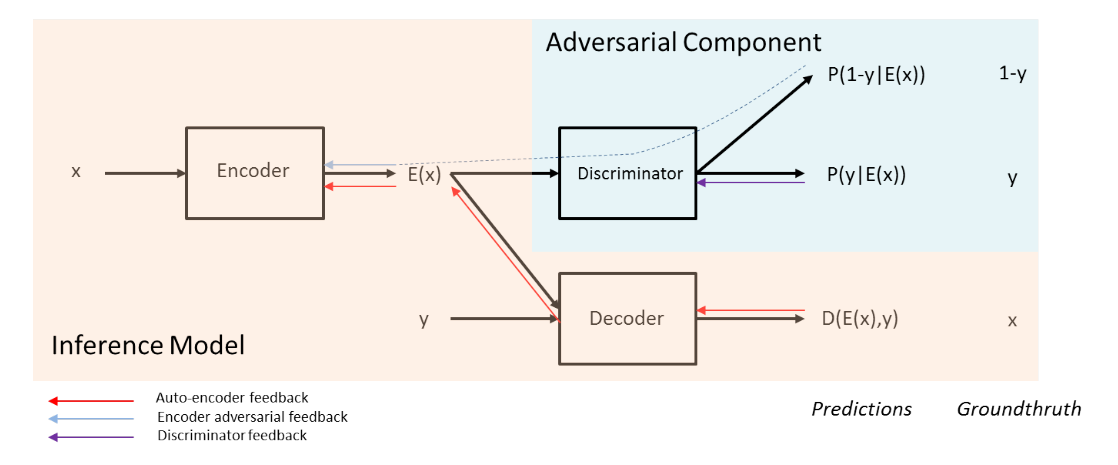
\includegraphics[width=0.9\textwidth]{images/fader-net.png}

\section{\citeall{Rezende2015VariationalFlows}}

\href{http://www.ipam.ucla.edu/abstract/?tid=16242&pcode=MLPWS1
}{IPAM Lecture Video} by Laurent Dinh from Google/MILA.

The main idea comes from the transformation of variables $z \rightarrow z^{\prime}$ for probability distributions.

\begin{equation}
q\left(\mathbf{z}^{\prime}\right)=q(\mathbf{z})\left|\operatorname{det} \frac{\partial f^{-1}}{\partial \mathbf{z}^{\prime}}\right|=q(\mathbf{z})\left|\operatorname{det} \frac{\partial f}{\partial \mathbf{z}}\right|^{-1}
\end{equation}

They propose that by using a series of bijective tranformations $f_k$ one can get from a simple starting distribution i.e. gaussian to a complicated one that explains the data.

\begin{equation}
\begin{aligned}
\mathbf{z}_{K} &=f_{K} \circ \ldots \circ f_{2} \circ f_{1}\left(\mathbf{z}_{0}\right) \\
\ln q_{K}\left(\mathbf{z}_{K}\right) &=\ln q_{0}\left(\mathbf{z}_{0}\right)-\sum_{k=1}^{K} \ln \left|\operatorname{det} \frac{\partial f_{k}}{\partial \mathbf{z}_{k-1}}\right|
\end{aligned}
\end{equation}

The transformations must be invertible (bijective) for the sampling to work. To make the calculation of the determinant tractable they enforce triangular Jacobians.

\section{\citeall{Chen2018NeuralEquations}}

Ruthoto: the selling point of Neural ODEs is that you don't need to store anything in memory because during the backward pass you can integrate backwards in time. But in his lecture he showed that the backward integration does introduce errors \cite{Ruthotto2019DeepEquations}.

\section{\citeall{Yldz2019ODE2VAE:Networks}}

Its an extension of VAE. The VAE encodes and decodes the latent space. The Neural ODEs are used to "propagate" this latent space continuously. They also use a bayesian networks as prior in the VAE so they can model uncertainty. The Neural ODE part gives continuous instead of discrete dynamics, the bayesian network can model multiple trajectories (uncertainty).

%%%%%%
%%%%%% IPAM
%%%%%%

\section{IPAM - Deep Learning in the Physical Sciences, Kyle Cranmer}

\href{http://www.ipam.ucla.edu/abstract/?tid=14649&pcode=DLT2018}{Lecture Video} by Kyle Cranmer, NYU

Many areas of science have simulations based on some well- motivated mechanistic model. However, the aggregate effect of many interactions between these low-level components leads to an intractable inverse problem. The developments in machine learning and AI have the potential to effectively bridge the microscopic - macroscopic divide and aid in the inverse problem.
\begin{itemize}
   \item they can provide effective statistical models that describe macroscopic phenomena that are tied back to the low-level microscopic (reductionist) model
   \item generative models and likelihood-free inference are two particularly exciting areas
\end{itemize}

\begin{center}
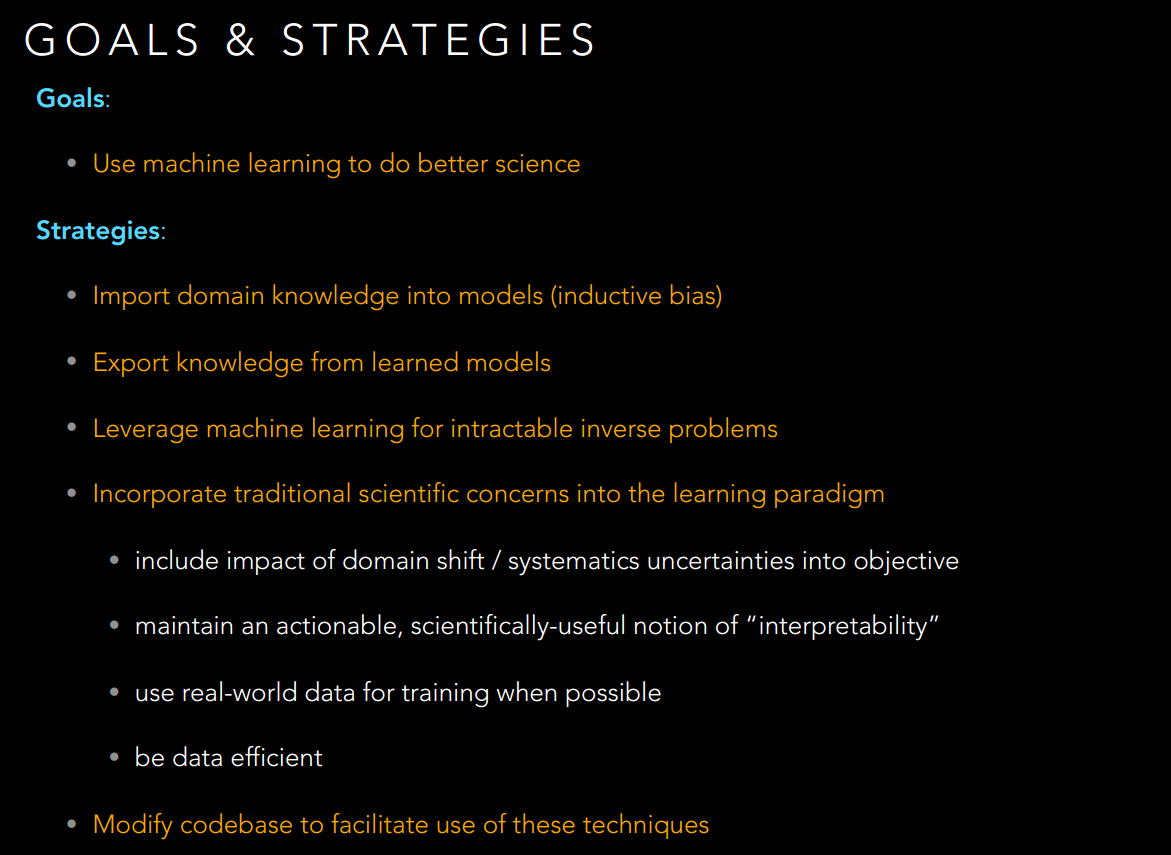
\includegraphics[width=0.8\textwidth]{images/goals-1.png}
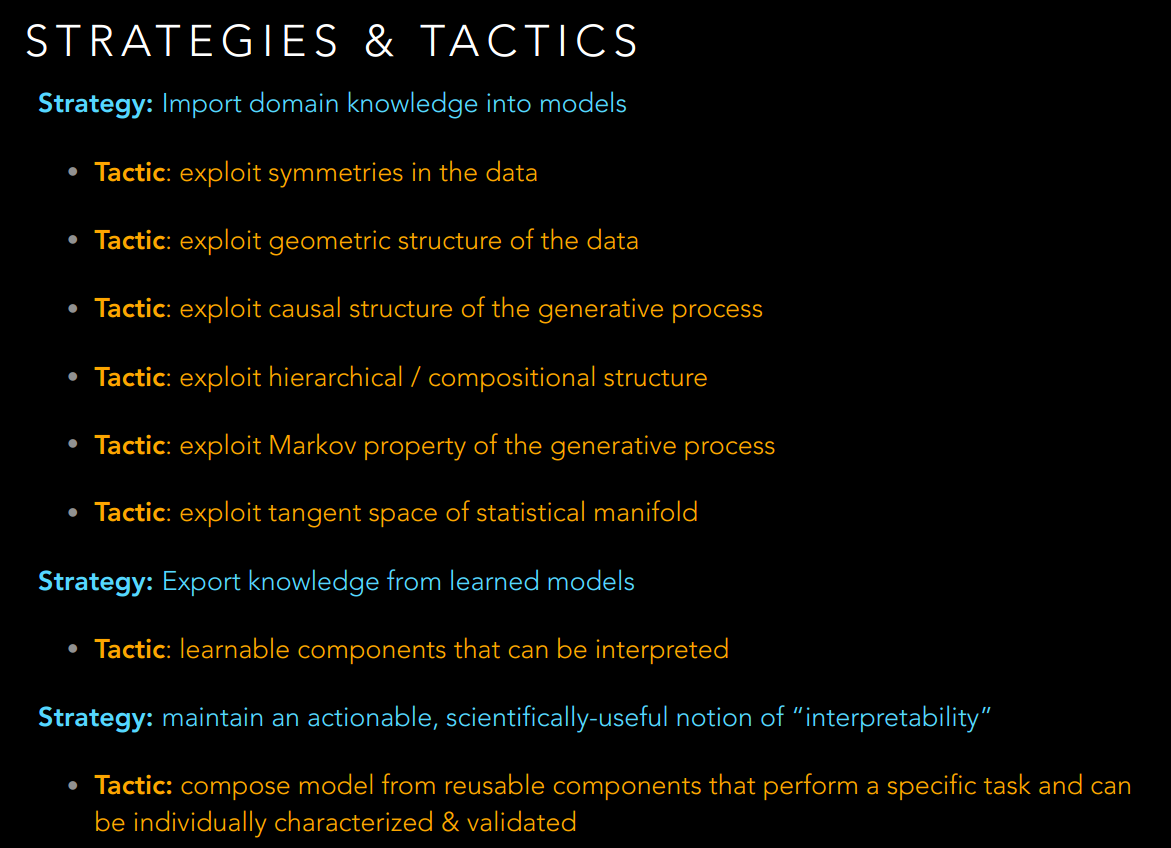
\includegraphics[width=0.8\textwidth]{images/goals-2.png}
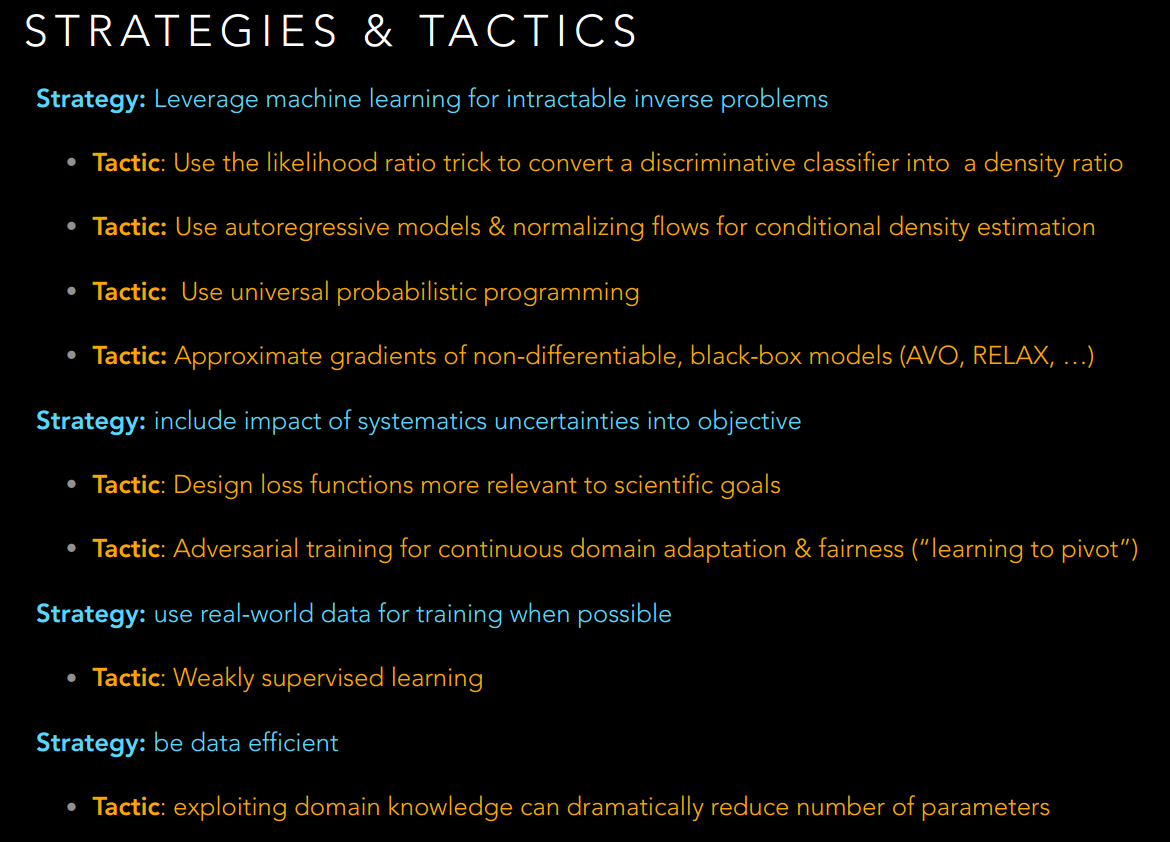
\includegraphics[width=0.8\textwidth]{images/goals-3.png}
\end{center}

\section{IPAM - Physics-Informed (and -informative) Generative Modelling in Astronomy, Joshua Bloom}

\href{http://www.ipam.ucla.edu/abstract/?tid=16152&pcode=MLPWS1}{Lecture Video} by Joshua Bloom from UC Berkeley.

How and why physics can be imbued in neural network models.

\begin{itemize}
    \item Symmetry. For example translational and rotational in-variance in convolutions.
    \item Bottlenecks enforce sparsity and Occam's razor.
    \item Loss function is physically meaningful per sample (i.e. reconstruction) but also for the whole generative model (i.e. distributional loss).
\end{itemize}

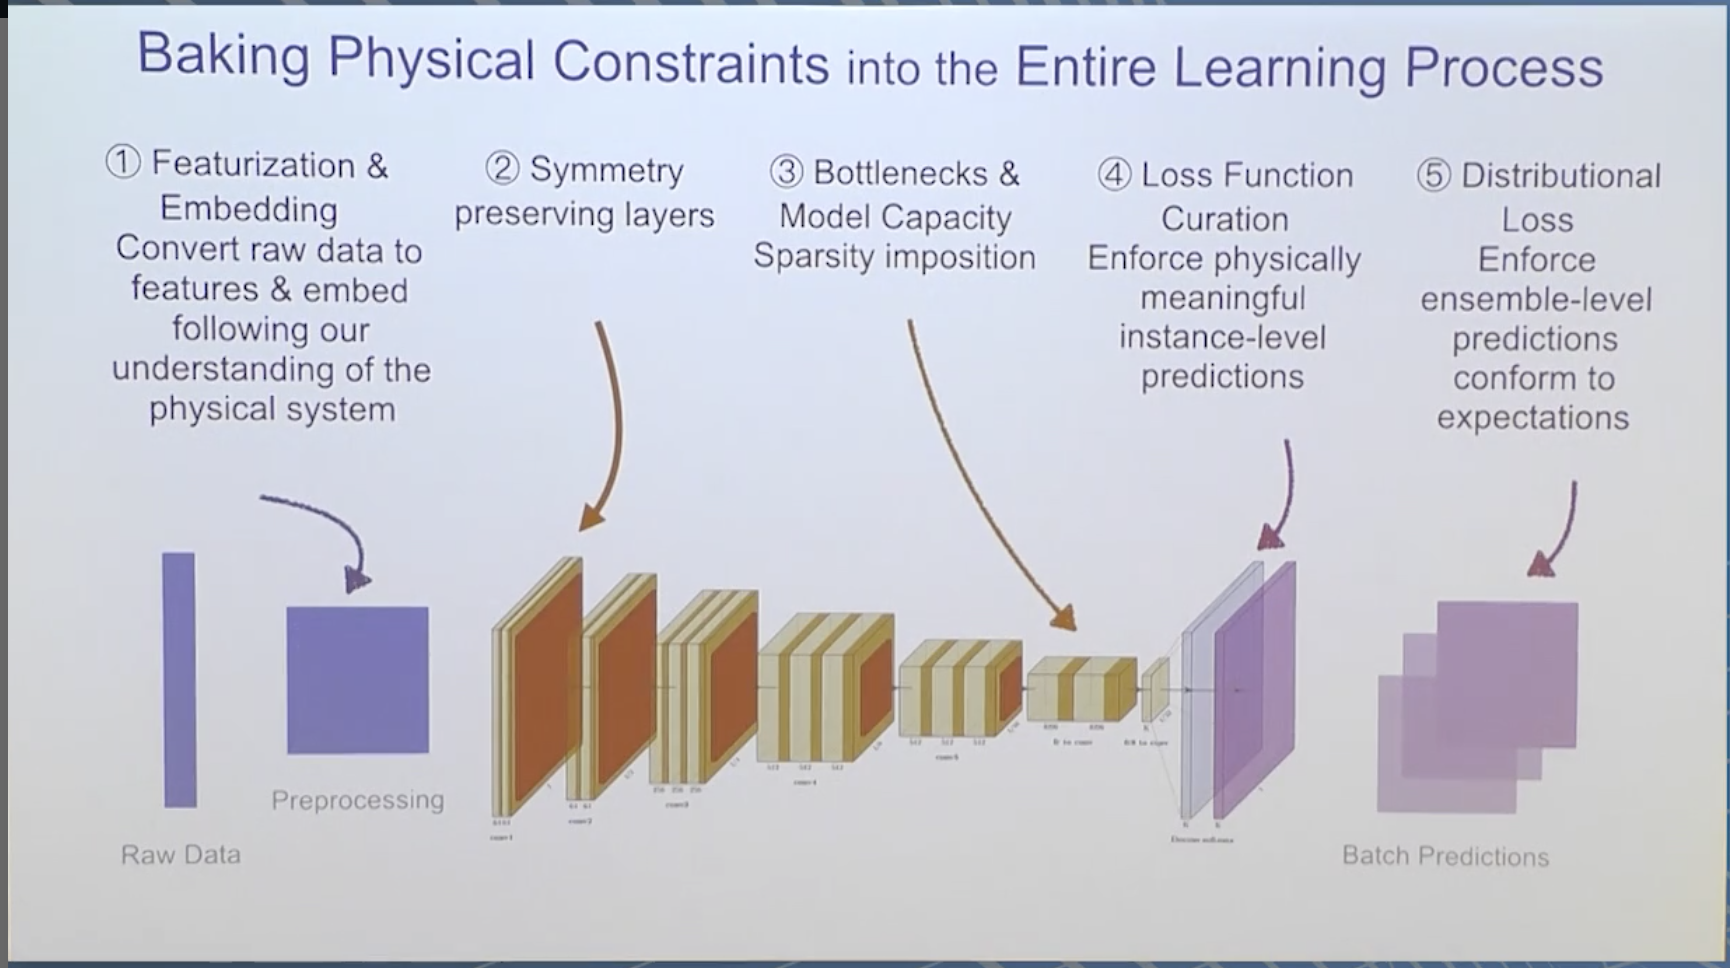
\includegraphics[width=0.9\textwidth]{images/Physics Inspired ML.png}

\section{IPAM - Deep Generative Learning for Physics Many-Body Systems, Frank Noe}

\href{http://www.ipam.ucla.edu/programs/workshops/workshop-i-from-passive-to-active-generative-and-reinforcement-learning-with-physics/?tab=schedule}{Lecture Video} by Frank Noe, Freie University of Berlin

An application of normalizing flows \parencite{Rezende2015VariationalFlows} and Real NVP \parencite{Dinh2016DensityNVP} in statistical physics. 

\section{IPAM - Deep Generative Networks as Inverse Generators, Stephane Mallat}

\href{http://www.ipam.ucla.edu/abstract/?tid=14547&pcode=DLT2018}{Lecture Video} by Stephane Mallat, Ecole Normale Superieure

\textbf{TL;DR} You can use priors to avoid learning a discriminator (GANs) or an encoder (VAEs) of generative network. 

\begin{itemize}
    \item Learning works well but you can formulate the problem as an inverse problem. This makes the problem tractable and allows for to incorporate all the prior information you know which is important for example in physics. Making the problem tractable means you can learn with less data.
\item Generators work like distributed (sparse) memories, they learn the pattern. The embedding has no information about the original patterns, it's a completely fixed operation. All the information is in the generator. What is the memory capacity of these networks?
\end{itemize}

\section{IPAM - Breaking Bad: Recent Advances from Function Space Characterization of Neural Nets with Implications for Physical Applications, Ankit Patel}

\href{http://www.ipam.ucla.edu/abstract/?tid=15765&pcode=MLPWS1}{Link to video}


Parametrization: After training you can reduce the parameters of a network by 95\% without loss of accuracy. Overparametrization is needed for learning but not for expressivity.

Lottery ticket hypothesis: The initial weights in some part of the network lead to good learning. Bigger networks have more chances. Alignment with overparametrization.  

Loss surface: High non-convexity but many local minima close to global minimum.

Generalization: Implicit regularization. For example adam vs sgd produce different generalization. Happens when the loss function is underdetermined.


\section{IPAM - A Numerical Analysis Perspective on Deep Neural Networks, Lars Ruthotto}
\href{http://www.ipam.ucla.edu/abstract/?tid=16362&pcode=MLPWS1}{Link to video}

ANODE paper Gholami et al 2019 exposes the challenges with Neural ODEs \parencite{Chen2018NeuralEquations}. Hamiltonian NN \parencite{Ruthotto2019DeepEquations}: You can get from input space to latent space and back, $X\rightarrow Z \rightarrow X$, without loss. Related to Reversible Net. 

Two ways to do optimal control. 
\uls
\li \textbf{First differentiate and then discretize.} First you solve the ODE forward in time and then based on the trajectory you solve another ODE backward in time. This other ODE is the adjoint equation and the process is similar to backprop. The adjoint is linearized so it is easier to solve. But the gradients you get from the adjoint are only useful if you solve forward and adjoint equations well. Because we work on a discretized domain.
\li \textbf{First discretize and then differentiate.} The PDE is discrete. We can use auto-grad to take the gradient out. The backprop gradients are often the same as what discretization of the adjoint equation would give, but not necessarily the ones for the "optimal" adjoint equation. The gradients are useful even if discretization is inaccurate. For example in the case of data with noise we don't need to solve the PDE with high accuracy because it is pointless.
\ule

\textbf{Why numeric methods for deep learning?}
\uls
    \li Transfer learning
    \uls 
        \li DL is similar to path planning, optimal control, differential equations.
    \ule
    \li Do more with less
    \uls
        \li Better data efficiency 
        \li 3D image and video classification? 
    \ule
    \li Power of abstraction. \uls \li Use contintuous interpretation to design and relate architectures. \ule
\ule

\section{IPAM - Recent advances in Derivative-Free Optimization and its connection to reinforcement learning, Katya Scheinberg}
\href{http://www.ipam.ucla.edu/abstract/?tid=15766&pcode=MLPWS1}{Link to video}

\uls
\li Derivative based optimization: we know the height and the slope. As if we are on a mountain.
\li Black-box optimization: we only know the value of our function. As if we are in the surface of the lake and measure the depth. The measurements are noisy.
\ule

Applications of derivative-free optimization:
\uls
\li Machine learning: binary loss function (1-0 loss). It is not black-box but the derivative is useless.
\li Deep learning: hyperparameter tuning
\li Reinforcement learning: policy gradients are gray-box, MCTS
\ule

Types of derivative-free methods: 

- Direct and random search

- Model based (interpolate sample points with linear or quadratic function)

For model-based we can use NNs. One assumption for convergence, the model should have comparable Taylor expansion as the true function w.r.t. to the step size. Quadratic models are better but cost should be taken into account. 

\uls
\li Interpolation allows previous points to be reused (sample efficiency)
\li Linear algebra can be expensive and ill-conditioned in high dims (RL)
\li Pre-designed sampling is is an option but incurs costs
\li Alternatives like Gaussian smoothing not necessarily better than pre-designed sampling
\ule

\section{\citeall{Cranmer2019LearningNetworks}}
\href{https://slideslive.com/38922576/learning-symbolic-physics-with-graph-networks}{NeurIPS ML4S video}

They look the problem of multi-body systems. The model they use is a graph network. They try to extract Netwon's laws from the network. The idea is as follows: in netwonian mechanics each body "feels" the force from each one of the other bodies. In graph networks each body can be a node and the force can be the vector message passed from one node the the other. If the dimension of the message vectors of the graph network is the same as the dimension of the force then after training they will be equal. Actually they find that the messages learn a linear transformation of Newton's laws.

To cope with unknown forces they use symbolic regression. Symbolic regression is a technique to find the proper formula to fit your data compining operations from a pool of operations like addition, multiplication, power etc. So, they approximate the force with symbolic regression on the messages. How do they find the correct dimension for the messages? They start with a higher dimension and reduce it until the error goes up (like the elbow method). 

They also found that lower dimensional messages generalize better to different number of bodies. 

\section{\citeall{Cranmer2019TheInference}}

\href{https://www.youtube.com/watch?v=odAQlcf5Urc}{Link to video}

Usually in Bayesian inference you want to calculate the posterior:
$$
p(\theta | x)=\frac{p(x | \theta) p(\theta)}{\int \mathrm{d} \theta^{\prime} p\left(x | \theta^{\prime}\right) p\left(\theta^{\prime}\right)}
$$

There are two sources of intractability for bayesian inference. The first is when the evidence $p(x)$ is intractable. This is solved by MCMC and VI. The other, common in simulations, is the intractability of the likelihood $p(x|\theta)$. This is also known as likelihood-free inference. Two ways to solve is 1) Approximate Bayesian Computation (ABC) and 2) create a model of the likelihood with methods like histograms or kernel density estimation. ABC uses summary statistics to reject or accept samples from the likelihood.

\textbf{Shortcomings of likelihood-free (simulation based) inference:
}\uls
\li Sample efficiency. Curse of dimensionality means ABC does not scale well
\li Quality of inference. Using summary statistics leaves some statistical power on the table.
\li Amortization. KDE is amortized but ABC not. In ABC new data requires repeating most steps. 
\ule

\textbf{Three ways to improve from recent advances in neural networks:
}
\uls
\li Neural networks do not suffer from the curse of dimensionality. In inference they can be used as surrogate models.
\li Active learning can improve sample efficiency
\li Integration of auto-diff and probabilistic programming in the simulation code. Simulators are no longer black boxes.
\ule

Talks a lot about normalizing flows and similar models.

\textbf{REVISE AGAIN LATER}

\section{\citeall{Both2019DeepMoD:Data}}

\href{https://www.youtube.com/watch?v=Ml4EXS_MUBc}{Link to video}

Their idea is to use a combination of neural networks and symbolic regression to do ODE identification in the presence of noise. The way they do is by incorporating the symbolic regression *within* the neural network. 

The model works as follows. First a neural network predict $u$. Then with auto-diff they get $u_t$. Then they have a lexicon of all possible symbolic variables $\Theta$ and weight it with $\xi$. The loss function is the reconstruction MSE plus the error between the $u_t$ and $\Theta \dot \xi$ plus a regularization in $\xi$. This way the network does not only learn to reconstruct but also to discover the network. The L1 regularization promotes sparsity in the coefficients. 

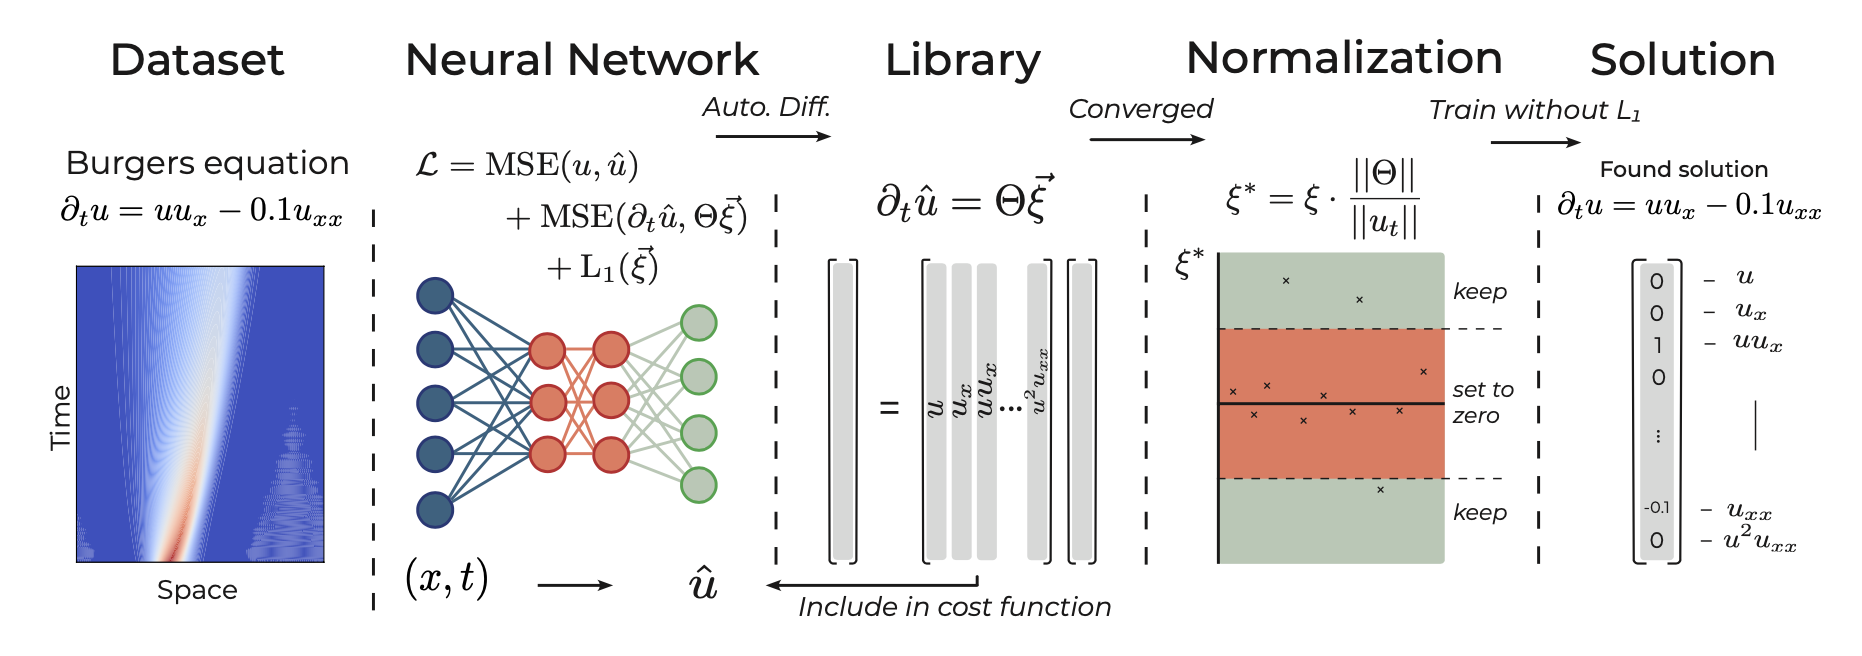
\includegraphics[width=0.9\textwidth]{images/deepmod.png}

They also have another paper named Temporal Normalizing Flows that does the system identification in PDEs \cite{Both2019TemporalFlows}.

\section{\citeall{Rezende2019EquivariantFlows}}

\href{http://youtube.com/watch?v=8VV0kL7Qg3Y}{Link to video 1}

\href{https://slideslive.com/38922578/equivariant-hamiltonian-flows}{Link to video 2}


This paper tries to conserve invariance when normalizing flows are used to transform distributions. Suppose a base distribution $\pi(z)$ is invariant with respect to a group of transformations. If we transform this density via a generic normalizing flow $f(z)$, there will be no guarantees that the transformed density $p(z)=\pi(f^{−1}(z))/det Jac$ will be invariant as well.
To do that they introduce equivariant Hamiltonian normalizing flows. The Hamiltonian is a function $H: \mathbb{R}^{2 d} \rightarrow \mathbb{R}$. They use two NNs one for the potential and another for the kinetic. They seperate the NNs because they use a symplectic integrator. 

Assume the data have a knowν symmetry generator. In order to apply a Hamiltonian flow on it they want to preserve the symmetry. To do that they use a regularizer between the flow and the symmetry generator. The regularizer is the Poisson bracket which for two scalar functions $f,g$ is:
$$
\{f(q, p), g(q, p)\}=\sum_{i} \frac{\partial f(q, p)}{\partial q_{i}} \frac{\partial g(q, p)}{\partial p_{i}}-\frac{\partial f(q, p)}{\partial p_{i}} \frac{\partial g(q, p)}{\partial q_{i}}
$$

The Hamiltonian coordinates and momentum in this method is not observable in the data. What one can do is treat the momentum variables p as latent. These variables has to be marginalized, as in Hamiltonian MC. To do that they use a variational approximation and optimize for VLB.

\section{\citeall{Sanchez-Gonzalez2019HamiltonianIntegrators}}
\href{http://www.ipam.ucla.edu/abstract/?tid=16226&pcode=MLPWS2}{Link to video}

\uls
\li Simulator: predicts next step from current by applying physics.
\li DeltaGN: it predicts the deltas for momentum and position. It's like an Euler scheme.
\li OGN: use a graph network to predict the derivatives and feed it to an integrator to predict.
\li HOGN: use a GN to predict the Hamiltonian energy H. Then differentiate that with auto-diff wrt to the input and treat is as a Hamiltonian. Then feed it to a symplectic integrator.
\ule

OGN and HOGN generalize better to time steps they have not been trained upon. They did two experiments one with fixed timestep and another where the timestep came from a range and they were feeding this timestep value with the input.

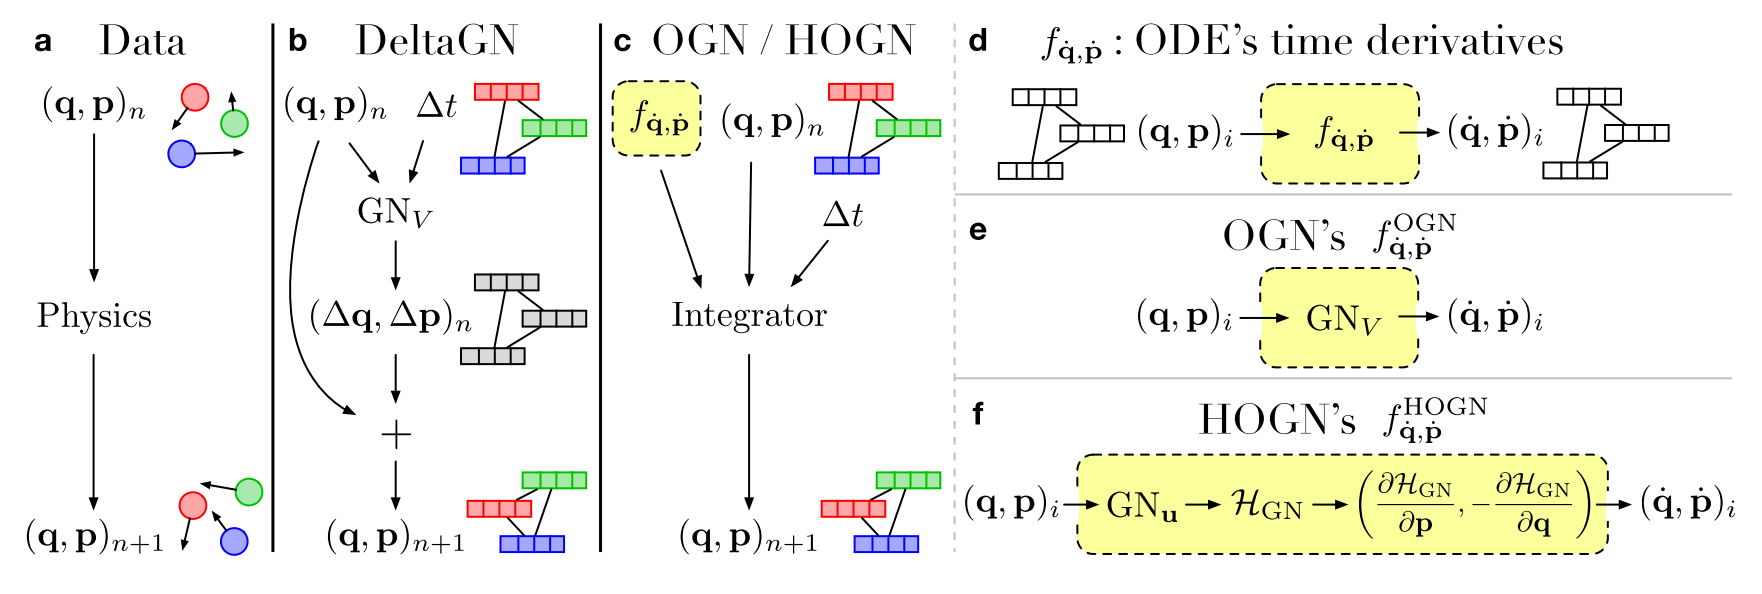
\includegraphics[width=0.9\textwidth]{images/hamgraph.png}

\section{\citeall{Sanchez-Gonzalez2018GraphControl}}

Interesting things about poking the system to infer latent variables with physical meaning like mass etc. These can be later used for downstream tasks. The system can be learned end-to-end.

The question is what actions lead to optimally identify the latent variables?

Another interesting thing is the pre-trained model can be used for model predictive control. MPC is when you have a model and then optimize for the controls that will give you a desired trajectory. There is no policy, the learned model serves as a forward model for simulation. The cool thing with GN is that it can be applied to multiples systems because it does pairwise predictions. This can be scaled to arbitrarily many pairs.

Also interesting things with predicting a multi-agent environment. Taccheti et al 2019.

\section{“Etalumis: Bringing Probabilistic Programming to Scientific Simulators at Scale.” Gunes Baydin et al. 2019}

\href{https://www.youtube.com/watch?v=aCh_n2yzSRc}{Link to video}
\href{http://www.ipam.ucla.edu/abstract/?tid=16191}{Link to video}

They combine simulators with probabilistic programming for inverse problems. 

\section{\citeall{Shanahan2019AnArchitecture}}

The use attention to extract "points of interest" from an image and then learn the relations of those points. The architecture is similar to Multi Head Attention \cite{Vaswani2017AttentionNeed} and close to a previous paper in Deep RL. They find that training on a relational task and then freeze the network helps with learning a new task (they only train the last part of the net). The attention learns to focus on the objects mostly. Also the representation they learn captures meaningful properties of the objects (after PCA), ie distinguishes between color & shape. Lastly their network can output symbolic propositions, prolog style, and these propositions can be queried from symbolic programming (prolog), although what these propositions mean is unclear. 

This work is related to graph networks but there we have the objects identified from a previous task, or they are given. This method identifies its own "objects" with attention. Also the work is relevant to symbolic/relational reasoning and AI.

Related review paper is \cite{Garnelo2019ReconcilingRelations}:
\textit{"In sum, there is a spectrum of approaches to compositionality, ranging from methods that engineer compositional structure directly into the representations to meth- ods that allow compositionality to emerge from the learning process in response to compositional structure in the data. Mid-way along this spectrum we find recent work on autoencoders whose loss functions promote com- positional representation."}

\section{\citeall{Brunton2016DiscoveringSystems}}

\href{http://www.ipam.ucla.edu/abstract/?tid=15783&pcode=MLPWS2}{IPAM WS2 video}

They do system identification in ODEs and PDEs from noisy data. They do sparse regularization to come up with only a few terms in each case. In the video he explains that you first can do a transformation that will linearize your system. This is the theory behind Koopman Operators but they are hard to find. By using NN they can jointly linearize the system and find its equations at the same time. 

\section{Adjoints and their applications, P. Farrell}

\href{dolfin-adjoint.org/en/latest/documentation/maths/index.html}{Link}

Let's say you want to design a wing with a low lift-to-drag ratio $J$ given some configuration of the wing parameterized by $m$. The physics of the systems are described by a systems of PDEs $$F(u,m)=0$$. By solving this equation we get a solution $u \in R^U$. For each set of parameters $m$ we get a solution, so $u$ is implicitly a function of parameters $u(m)$. The set of PDEs pose a constraint on the optimization problem over $J$. So one way to go about this is to treat the PDE solver as a black box and solve for a functional \textit{functional} $$\widehat{J}(m)=J(u(m),m)$$. The problem is that since the solver is a black box to use, we only have the values of $\widehat{J}$ without its derivative. Thus we can only use derivative-free optimization such as genetic algorithms. Derivative-free optimization methods do not scale well with dimensions and can take a lot of iterations to converge. If we have derivative info for $\widehat{J}$ we can converge one or two orders of magnitude faster. There are three main ways to compute derivatives: Finite differences, tangent linear approach and the adjoint method.

\subsection{Finite differences }
These are straightforward: 
$$
\frac{\mathrm{d} \widehat{J}}{\mathrm{d} m_{i}} \approx \frac{\widehat{J}\left(m+h e_{i}\right)-\widehat{J}(m)}{h}
$$

\subsection{Tangent linear approach}
Applying chain rule to the functional $\widehat{J}(m)=J(u(m), m)$ gives:
$$\frac{\mathrm{d} \widehat{J}}{\mathrm{d} m}=\frac{\partial J}{\partial u} \frac{\mathrm{d} u}{\mathrm{d} m}+\frac{\partial J}{\partial m}$$
The hard part here is the Jacobian matrix $du/dm$ with dimensions $U\times M$ (solution space x parameter space).
We can find a solution implicitly by differentiating $F(u,m)=0$ wrt $m$.
$$
\begin{array}{0}\frac{\mathrm{d}}{\mathrm{d} m} \boldsymbol{F}(u, m)=\frac{\mathrm{d}}{\mathrm{d} m} 0 \\ \frac{\partial F(u, m)}{\partial u} \frac{\mathrm{d} u}{\mathrm{d} m}+\frac{\partial F(u, m)}{\partial m}=0 \\ \frac{\partial F(u, m)}{\partial u} \frac{\mathrm{d} u}{\mathrm{d} m}=-\frac{\partial F(u, m)}{\partial m}\end{array}
$$

The last equation is called the \textbf{tangent linear equation}. The unknown is $du/dm$. The term $\partial F(u, m) /  \partial u$ is a matrix $U\times U$ so it's actually a linear operator around the solution $u$, no matter if $F(u,m)$ is linear or not. Similarly $\partial F(u, m) /  \partial m$ is a matrix $U\times M$. This term acts as a source term, each column of  $\partial F(u, m) /  \partial m$ provides the source term for the derivative over $u$. Notice that the functional $J$ does not appear at all. For a given parameter (input), the tangent linear solution can be used to easily compute the gradient of any functional. This means that solving the tangent linear system makes sense when there are a small number of parameters (inputs), and a large number of functionals of interest (outputs).

\subsection{Adjoint method}

Suppose the tangent linear system is invertible. Then we can rewrite the solution Jacobian as:

\begin{equation}
\frac{\mathrm{d} u}{\mathrm{d} m}=-\left(\frac{\partial F(u, m)}{\partial u}\right)^{-1} \frac{\partial F(u, m)}{\partial m}
\end{equation}

So the derivative of the loss over the parameters becomes:

\begin{equation}
\begin{array}{l}\frac{\mathrm{d} \widehat{J}}{\mathrm{d} m}=\frac{\partial J}{\partial u} \frac{\mathrm{d} u}{\mathrm{d} m}+\frac{\partial J}{\partial m} \\ \frac{\mathrm{d} \widehat{J}}{\mathrm{d} m}=-\frac{\partial J}{\partial u}\left(\frac{\partial F(u, m)}{\partial u}\right)^{-1} \frac{\partial F(u, m)}{\partial m}+\frac{\partial J}{\partial m}\end{array}
\end{equation}

The adjoint is: 
\begin{equation}
\begin{array}{l}\lambda=\left(\frac{\partial F(u, m)}{\partial u}\right)^{-*} \frac{\partial J^{*}}{\partial u} \\ \left(\frac{\partial F(u, m)}{\partial u}\right)^{*} \lambda=\frac{\partial J^{*}}{\partial u}\end{array}
\end{equation}

% or 
% $$
% \frac{\partial J}{\partial m} = \lambda^T \frac{\partial F(u, m)}{\partial m})
% $$

\section{IPAM - Improving PDE solvers and PDE-constrained optimization with deep learning and differentiable programming}

\href{http://www.ipam.ucla.edu/abstract/?tid=16344&pcode=MLPWS2}{Link to video}

Combine approximation of neural networks with the domain knowledge of physical laws. Adding the physical laws can help with interpretability and generalization. By differential programming he means machine learning (auto-grad). They present two methods:

\subsection{\citeall{Bar-Sinai2019LearningEquations}}

This paper uses ML to find what discretization to use for solving PDEs. e.g. what coefficients to use in central approximation of derivatives:
$$
\begin{aligned} \frac{\partial^{2} v}{\partial x^{2}} & \approx \frac{v_{i+1}-2 v_{i}+v_{i-1}}{\Delta x^{2}} \\ & \approx \frac{-v_{i+2}+16 v_{i+1}-30 v_{i}+16 v_{i-1}-v_{i-2}}{12 \Delta x^{2}} \end{aligned}
$$

\subsection{Hoyer et al. Neural reparametrerization improves structural optimization.}

Deep Image Prior \cite{Lempitsky2018DeepPrior}: train a CNN to reconstruct just one image and this produce a super-resolution image. The idea is that the only optimize one example and for a limited amount of iterations. This for some reason works well for reconstructing the details. They use a similar approach.

\section{\citeall{Lempitsky2018DeepPrior}}

\href{https://medium.com/@ahmdtaha/deep-image-prior-7e0eac506dee}{Medium article}

\href{https://towardsdatascience.com/demystifying-deep-image-prior-7076e777e5ba}{Another medium article}

This work is about image restoration, denoising, inpainting etc. We denote the clean image as $x$, the degraded image as $\hat{x}$ and the restored image as $x^*$. We try to find:

$$
\mathrm{x}^* = \argmax_{\mathrm{x}}{p(\mathrm{x}|\dot{\mathrm{x})}}
$$

where: 

\begin{equation}
p(\mathrm{x} | \dot{\mathrm{x}})=\frac{p(\dot{\mathrm{x}} | x) p(x)}{p(\mathrm{x})} \alpha p(\dot{\mathrm{x}} | \mathrm{x}) p(\mathrm{x})
\end{equation}

hence: 

\begin{equation}
\begin{aligned} x^{*} &=\argmax_{\mathrm{x}}{p(\dot{\mathrm{x}} | \mathrm{x})} \\ 
&=\argmin_x -\log p(\dot{\mathrm{x}} | \mathrm{x})-\log p(\textbf{\mathrm{x}}) \\ 
&=\argmin_x E(x ; \dot{\mathrm{x}})+R(x) \end{aligned}
\end{equation}

In this case $E(x ; \dot{\mathrm{x}})$ is some reconstruction cost and the $R(x)$ is the image prior which works as a regularizer. Usually what you do is start from a random image and try to traverse the image space until you reach a good point. The reconstruction cost is task specific while the regularizer is some implicit or explicit prior about the distribution of images. Also the reconstruction can be learned end-to-end with a neural network from real images. This paper uses another method, instead of finding the reconstructed image it tries to find a neural network that starts with noise and creates a reconstructed image. They motivate this by saying that the NN is a surjective mapping from the parameters of the network $\theta$ to the image space $g(\theta) \rightarrow x$. They only take into account E and get rid of the regularizer. The method is feeding noise to a U-Net and make it reconstruct the corrupted image. If you train it for a long time it will reconstruct the noisy image but if you stop early then the image you get is pretty close to the original one. It is not clear when to stop, other methods tried to find heuristics on that (check link 1 above). This paper indicates that the structure of the CNN is a good prior for images by itself.

\section{\citeall{Bengio2019AMechanisms}}

The authors define "a meta-learning objective that measures the speed of adaptation, i.e., a form of regret, in order to optimize the way in which knowledge should be represented, factorized and structured ... this way, we can take what is normally considered a nuisance in machine learning (changes in distribution due to non-stationarity, uncontrolled interventions, etc.) and turn that into a training signal to find a good way to factorize knowledge into components and mechanisms that match the assumption of small change. "

Imagine we have a system that produces data. A change in the system (interventioin) causes a non-stationarity in the produced data and their distribution changes. This is a common setup in supervised learning where the testing data are different from the training data. Let say that the system has two parts, one that changes after the intervention and another part that stays the same. If our model can capture this it would be easier to adapt.

This can be depicted in a graphical model with two nodes A,B. In this case the joint distribution is $P(A,B) = P(A|B)P(B) = P(B|A)P(A)$, both factorizations are valid. Imagine that we change the distribution $P(A)$ through an intervention. This imposes implicitly a specific causal structure to the model where $A \rightarrow B$ (A is the parent of B) and only one of the factorizations is actually true. So if a neural network learns the original distribution $P(A,B)$ after the change in $P(A)$ it needs to re-learn the new distribution. The authors say that if the NN learns the correct causal structure $P(A,B) = P(B|A)P(A)$ then after an intervention in $P(A)$ it should be able to meta-learn faster than the model with the opposite structure. Experimentally, they demonstrate that indeed the correct model learns faster in a meta-learning setting. They also construct a formulation of regret, i.e. how fast a network meta-learns. They show that this indicates the correct model, opening the avenue to learn a causal model from the data directly, in this simple scenario.  

\section{\citeall{Vaswani2017AttentionNeed}}

\href{http://www.peterbloem.nl/blog/transformers}{Link to article}

This is best understood in a language modeling setting. We have a sequence of words. Each word has an embedding (we learn it), also each word can have a positional embedding, also learned. Then there is the attention module which has three matrices Q, K, V:

\begin{equation}
\text { Attention }(Q, K, V)=\operatorname{softmax}\left(\frac{Q K^{T}}{\sqrt{d_{k}}}\right) V
\end{equation}

Where k is the dimension of the embedding. We can also have multi head attention where each head applies to the input sequence seperately. There many variations on how to learn the various heads, in the original paper they learn linear transformations of Q,K,V for each head but we can also learn separate matrices for each head.

\begin{equation}
\begin{array}{l}\qquad \begin{aligned} \text { MultiHead }(Q, K, V) &\left.=\text { Concat (head }_{1}, \ldots, \text { head }_{\mathbf{h}}\right) W^{O} \\ \text { where head }_{\mathbf{i}} &=\text { Attention }\left(Q W_{i}^{Q}, K W_{i}^{K}, V W_{i}^{V}\right) \end{aligned} \end{array}
\end{equation}

 \text { Where the projections are parameter matrices } W_{i}^{Q} \in \mathbb{R}^{d_{\text {model }} \times d_{k}}, W_{i}^{K} \in \mathbb{R}^{d_{\text {model }} \times d_{k}}, W_{i}^{V} \in \mathbb{R}^{d_{\text {model }} \times d_{v}} \\ \text { and } W^{O} \in \mathbb{R}^{h d_{v} \times d_{\text {model }}}.  
 The $W^0$ does the final aggregation of the heads, see figure below.

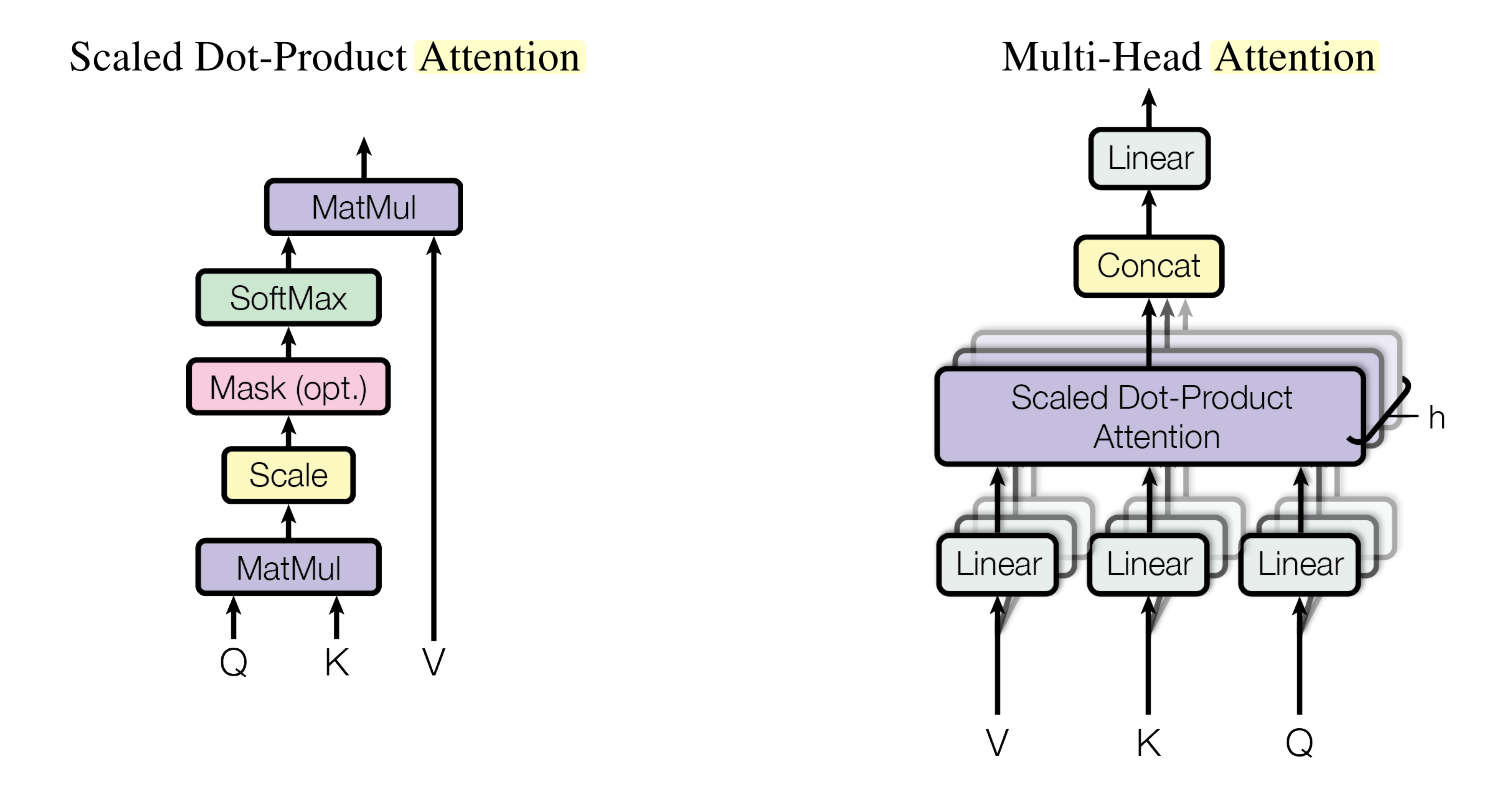
\includegraphics[width=0.8\textwidth]{images/attention.png}

Below we see a typical transformer networks. This is the sequence: a self attention layer, layer normalization, a feed forward layer (a single MLP applied independently to each vector), and another layer normalization. Residual connections are added around both, before the normalization. The order of the various components is not set in stone; the important thing is to combine self-attention with a local feed forward, and to add normalization and residual connections. (from article link)

\includesvg[width=0.8\textwidth]{images/transformer.svg}

Basic intuitions:

\uls
\li The word embedding that are more relevant will give a higher score.
\li The context is important that's why we sum all over it.
\li In RNNs we have to do serial computation but in Transformer this is not a problem we can run a whole sentence in parallel.
\li In constrast with convolutions we have all the context at hand, we don't need repeated layers that use stride/downsampling that dilutes the signal
\ule

\section{\citeall{Scholkopf2019CausalityLearning}}

He makes the point between statistical and causal dependence, which is the analogous of correlation is not causation. Argues that causality is needed for generalization. When the IID assumption is violated (dataset shift) then statistical methods fails. A causal model contains more info that a statistical one because it contains the dependencies between the variables. 

The \textbf{Common Cause Principle} says that if two vars are dependent then there is another one that causally influences both. The main modelling tool for causal graphs are the\textbf{ Structural Causal Models (SCM)}. The idea is that instead of have parent-child relationships $P(X_i|PA_i)$ we model the variables as functions $X_i := f_i(PA_i, U_i)$, where U is a stochastic unexplained variable (noise). The set of noises $U_1, \elipsis U_n$ are jointly independent. The SCM allows for interventions in U or f (ie set it constant). We can write the causal factorization: 

\begin{equation}
p\left(X_{1}, \ldots, X_{n}\right)=\prod_{i=1}^{n} p\left(X_{i} | \mathbf{P A}_{i}\right)
\end{equation}

Statistical learning tries to find a joint of the data, causal learning seeks to exploit the fact that the joint distribution possesses a causal factorization. 

Taxonomy of models depending on the detail. 

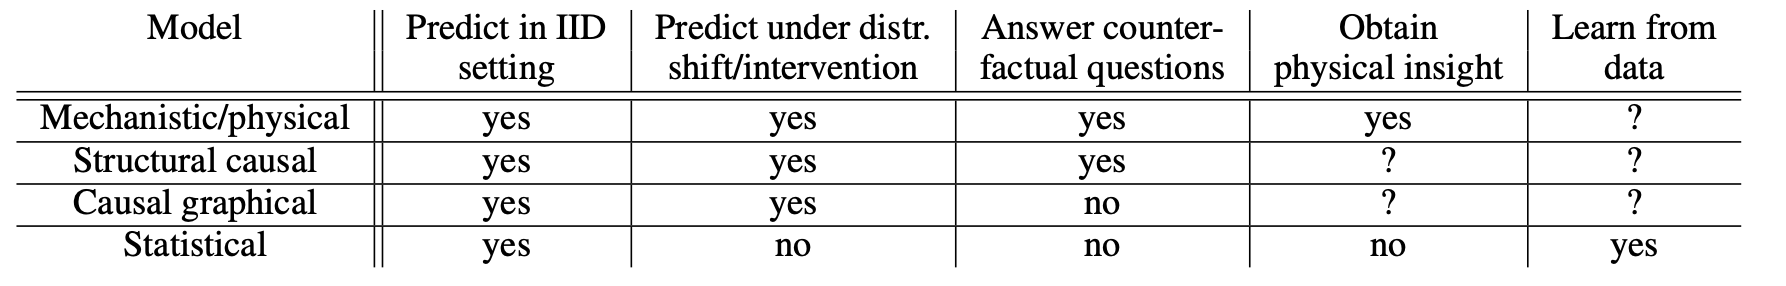
\includegraphics[width=0.9\textwidth]{images/causal_taxonomy.png}

\textbf{Independent Causal Mechanisms (ICM) Principle.} The causal generative process of a system’s variables is composed of autonomous modules that do not inform or influence each other.
In the probabilistic case, this means that the conditional distribution of each variable given its causes (i.e., its mechanism) does not inform or influence the other mechanisms. Our brains think that an object is independent of the mechanism that gives us the information about said object. This is called invariance. 

\textbf{Causality in representation learning.} In SCM the noise is exogenous, similar to how the noise is treated in VAEs, both use the reparametrization trick. Various directions.\textit{ Learning transferable mechanisms:} the world is modular we can learn independent causal mechanisms. This can be done with competitive training \cite{Goyal2019RecurrentMechanisms}. \textit{Learning disentangled representations:} Intervening upon latent variables. One way to intervene is to replace noise variables with the corresponding values computed from other input images, a procedure that has been referred to as hybridization by Besserve et al. (2018b). \textit{Learning interventional world models and reasoning} Causality will play a role in representation learning and maybe self-consiousness might need to be represented in the latent variables.

\section{\citeall{Goyal2019RecurrentMechanisms}}

Their idea is that a complex generative model, temporal or not, can be thought of as the composition of independent mechanisms or “causal” modules. They use multiple LSTMs each one with each own attention mechanism which they call Recurrent Independent Mechanisms. Since the queries depend on the state of the RIMs, this enables individual RIMs to attend only to the part of the input that is relevant for that particular RIM, thus enabling selective attention based on a top-down attention process. They promote the competition between RIMs for the final output by keeping the "highest rated" RIMs for each input. They also allow communication between RIMs by allowing the activated RIMs to read from all other RIMs (activated or not). The intuition behind this is that non-activated RIMs are not related to the current input, so their value should not change. However they may still store contextual information that is relevant for activated RIMs. 

\section{\citeall{VanSteenkiste2019AreReasoning}}

In previous work \cite{Locatello2018ChallengingRepresentations} they had found that disentanglement did not provide better results in downstream tasks. But it was a very simple taks. In this work they look deeper and find that disentanglement indeed helps with downstream tasks. They are considering relations reasoning tasks like dSprites and 3dshapes. This paper is a huge study of 360 unsupervised models from 4 different disentanglement approaches (beta-VAE, FactorVAE, beta-TCVAE, and DIP-VAE). The disentangled representations are then used to train Wild Relational Networks. They report "compelling evidence that more disentangled representations yield better sample-efficiency in learning to solve the considered abstract visual reasoning tasks".

\section{\citeall{Arjovsky2019InvariantMinimization}}

Interesting experiment: split MNIST datasets in two, from 0-4 and 5-9. The labels have 25\% error so a perfect classifier can only be 75\% correct. Then we color both classes in different color (low numbers green, high numbers red). The color labels have also noise 0.1 or 0.2 (two "environments"). A normal classifier would take advantage of the color because the noise is less than the noise due to shape. But it would fail if during test the color noise is 0.9. A classifier that learns the invariant causes of the data i.e. the shapes would be more robust. Invariance across environements buys extrapolation powers. But this is not straightforward how to do it in realizable problems (that is when the noise in labels is small and the classifier can get close to optimal performance). 

The statistical problem is a proxy of the real problem, there is a gap we haven't explored. Nature does not shuffle, by shuffling we remove useful information, mainly the info that is stable and invariant. When you are optimal for multiple environments and linear combinations of them then possibly you can extrapolate. Invariance is closely related to causation. Whithout noise it's trickier.

Difference to domain adaptation. In DA you know the target domain and you also don't care about the output labels. DA is for covariate shift, ie diss of X and Y change together, in IRM distribution over X stays the same but changes for Y.

\section{\citeall{Lu2019UnderstandingView}}
Transformer as ODE Conv-Diff solver.

\section{\citeall{Mooij2013FromCase}}

The formulate structural equations where the derivatives of a variable depend on its parent variables in a structural causal model (SCM). This model also has corresponding equilibrium equations. They say that an SCM can model an ODE. But SCM there are no loops while in ODEs a derivative of a variable can depend on the value of the same variable. They say that the solution is implicit by the structural stability solutions:

$$
\begin{array}{l}\text { Note that even though the ODE may contain self- } \\ \text { loops (i.e., the time derivative } \dot{X}_{i} \text { could depend on } \\ X_{i} \text { itself, and hence } \left.i \in \operatorname{pa}_{\mathcal{D}}(i)\right), \text { the induced SCM } \\ \mathcal{M}_{\mathcal{E}_{\mathcal{D}}} \text { does not contain self-loops by construction (i.e., } \\ \left.i \notin \mathrm{pa}_{\mathcal{M} \varepsilon_{\mathcal{D}}}(i)\right) \text { . Somewhat surprisingly, the structural } \\ \text { stability conditions actually imply the existence of self- } \\ \text { loops (because if } X_{i} \text { would not occur in the equilibrium } \\ \text { equation }\left(\mathcal{E}_{\mathcal{D}}\right)_{i}, \text { its value would be undetermined and } \\ \text { hence the equilibrium would not be unique). }\end{array}
$$

\section{\citeall{Cranmer2020DiscoveringBiases}}

They look into physical systems that can be modeled as interacting nodes. They use graph networks to learn to predict those systems and regularize the message passing between the nodes. In systems like moving particles they show that the most important messages element $\phi_1^e$ (after regularization) corresponds to (a linear combination) of the real forces. 

They also use symbolic regression to predict $\phi_1^e$ from mass, positions of nodes, etc and are able to recover (not always) the underlying physical laws.


\section{\citeall{Saemundsson2019VariationalEmbeddings}}

The take the idea of Neural ODEs where neural networks are seen as discretized dynamical systems. They mix that with the viewpoint of geometric embeddings which impose structure on an embedding space. Instead of the Euler scheme and make use variational integrators, a class of discretization methods that respect and preserve the underlying geometry of a physical system.

\section{\citeall{Greydanus2019HamiltonianNetworks}}

They parametrize the Hamiltonian H of a system with a neural net. They use autograd and Hamilton's equations to predict the derivatives of the phase space:
$$
\frac{d \mathbf{q}}{d t}=\frac{\partial \mathcal{H}}{\partial \mathbf{p}}, \quad \frac{d \mathbf{p}}{d t}=-\frac{\partial \mathcal{H}}{\partial \mathbf{q}}
$$

Then they use an Euler integrator to find the next point in the phase space.

\section{\citeall{Toth2019}}

They use a network to deduct a latent space from pixel observations (multiple frames). They unroll this latent space to the future using the Hamiltonian equations. The latent space is not 2-dimensional (like the phase space) but higher. The motivation is that respecting the Hamiltonian in the latent space will preserve energy. They use a leapfrog (symplectic and energy preserving) integrator.

\section{\citeall{Higgins2018TowardsRepresentations}}

Still absorbing.

They formulate the disentanglement of factors of variation in the generative process that creates the data. The formulation is based on group theory and the decomposition of group actions in subgroups. Interestingly the rotation around the cartesian axes can not be decomposed in subgroup actions. 

"In machine perception, the most powerful generalisation we can hope for is by understanding what properties of the world remain the same when transformed in certain ways."

\section{\citeall{Locatello2019DisentanglingLabels}}

They study how some labels on the factors of variation can help with model selection and semi-supervised learning. In the case of SS learning they use the labels to learn the factors of variation in the latent space. They normalize them in [0,1] and also do some binning (need to read more on how to treat continuous factors).

Some good pointers for other types of inductive biases for disentanglement such as:

\begin{quote}
Other forms of inductive biases such as relying on temporal information (video data) (Denton and Birodkar, 2017; Yingzhen & Mandt, 2018), allowing for interaction with the environment (Thomas et al., 2017), or incorporating grouping information (Kulkarni et al., 2015; Bouchacourt et al., 2018) were discussed in the literature as candidates to circumvent the impossibility result by Locatello et al. (2019b)
\end{quote}


\section{\citeall{Locatello2018ChallengingRepresentations}}

They say that disentanglement cannot be achieved without inductive biases in the model or the data (labels). They provide some concise description of disentanglement metrics in the appendix.

\section{\citeall{Miladinovic2019DisentangledRepresentations}}

They want to solve the problem of different dynamics in ODEs and in general (similar to ours). 
$$
P^{D_{k}}\left(X_{i} \mid \vec{X}_{<i}\right) \neq P^{D_{m}}\left(X_{i} \mid \vec{X}_{<i}\right), for k \neq m
$$

The formulation for the model is a bayesian DGM as a state-space model. Where the dynamics D are inferred prior to the sequence prediction (and affect all steps of the prediction). The idea in SSMs is that the next prediction is found by unrolling the state-space and decoding it. The also model noise in the latent space unrolling and the reconstruction/decoding.

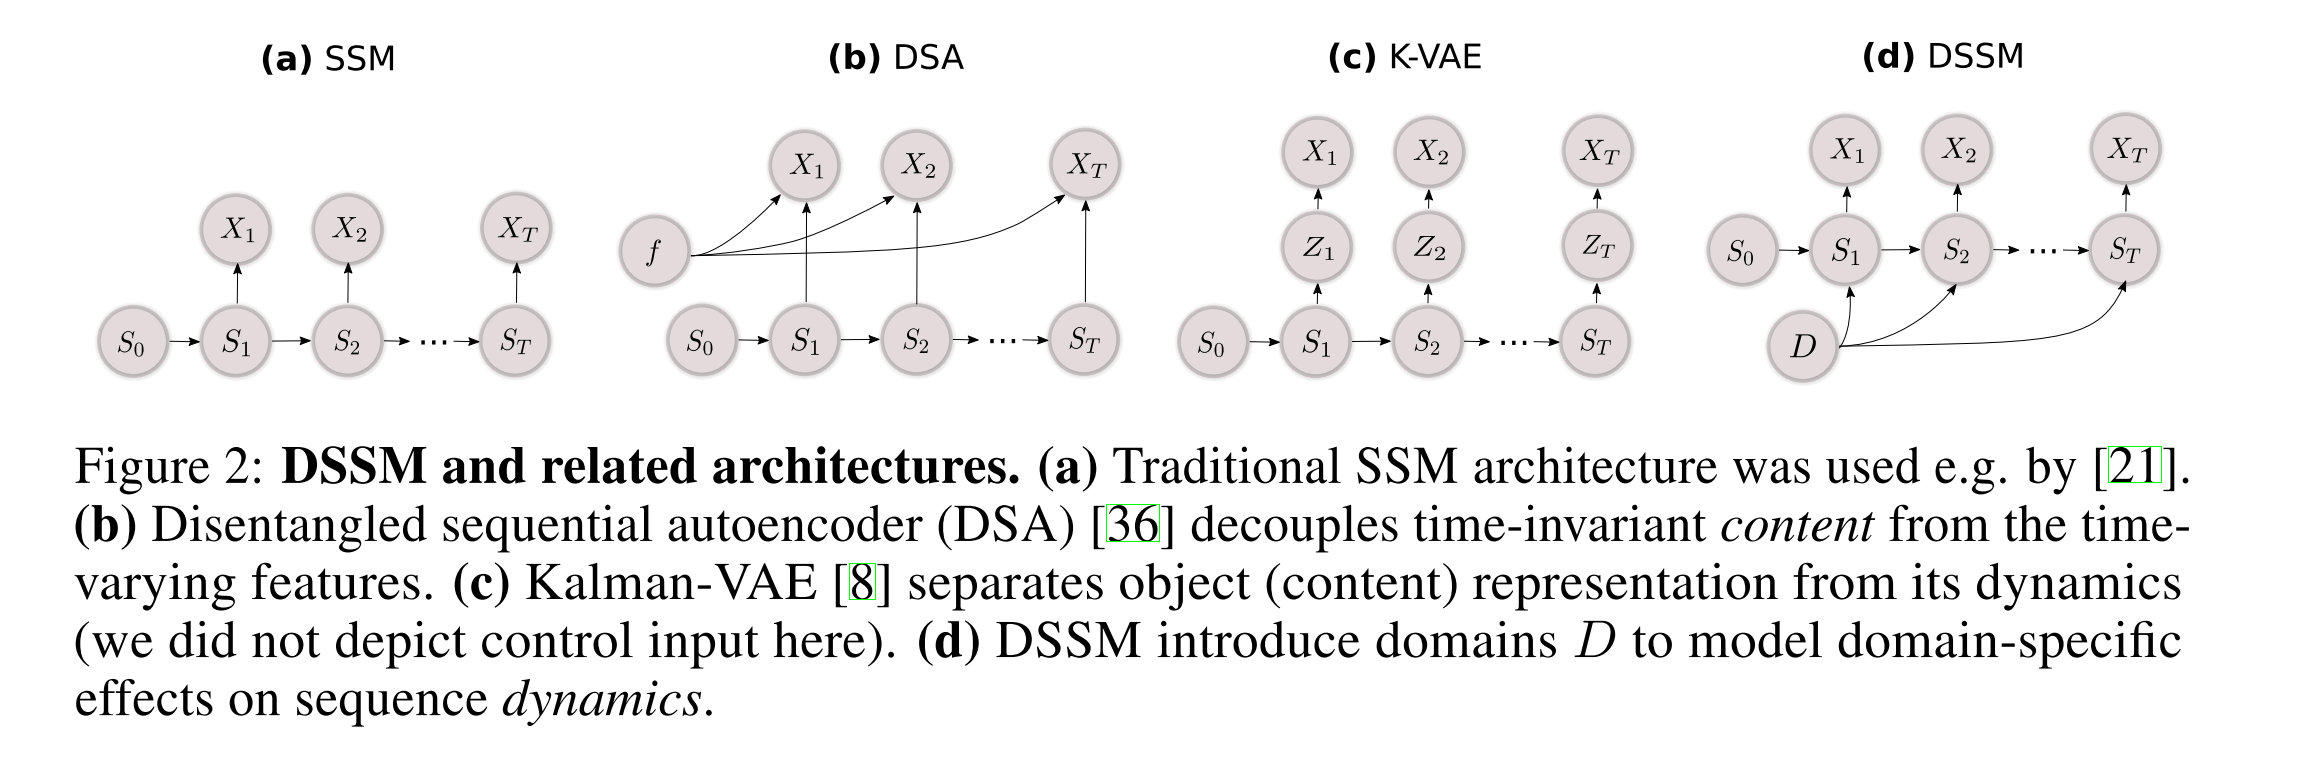
\includegraphics[width=0.8\textwidth]{images/dssm.png}

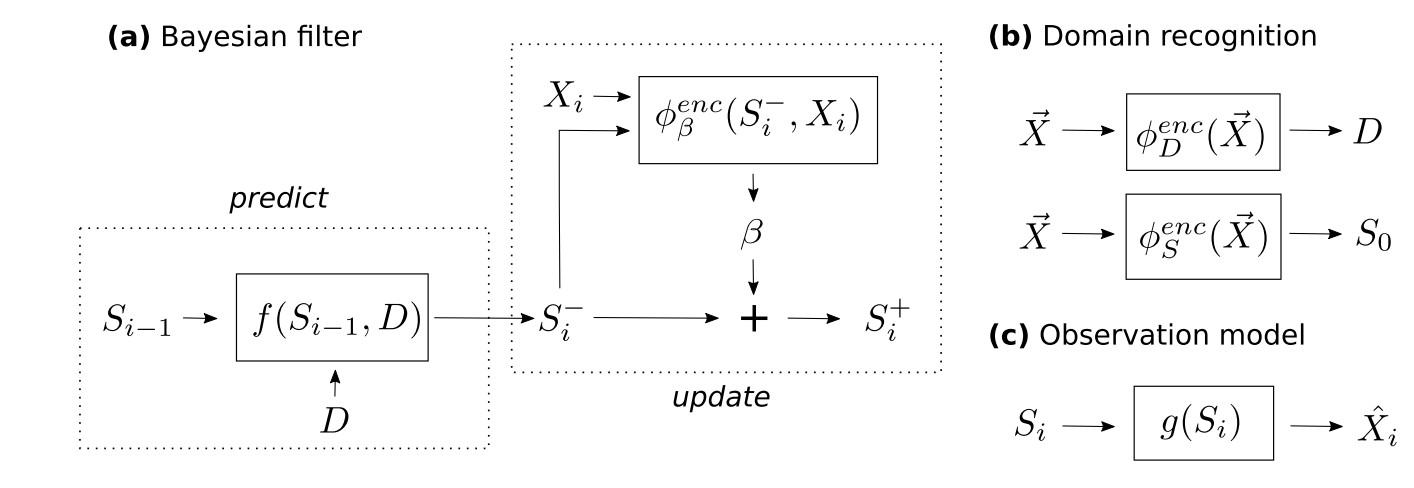
\includegraphics[width=0.8\textwidth]{images/dssm2.png}

\section{\citeall{LeGuen2020DisentanglingPrediction}}

They disentangle the dynamics (movement) from the details (texture, appearance). The PhyCell models the physics and the ConvLSTM the details. PhyCell has a predictor and correction scheme (similar to DSSM that models noise). The predictor is based on convolutions that combine spatial derivatives. 

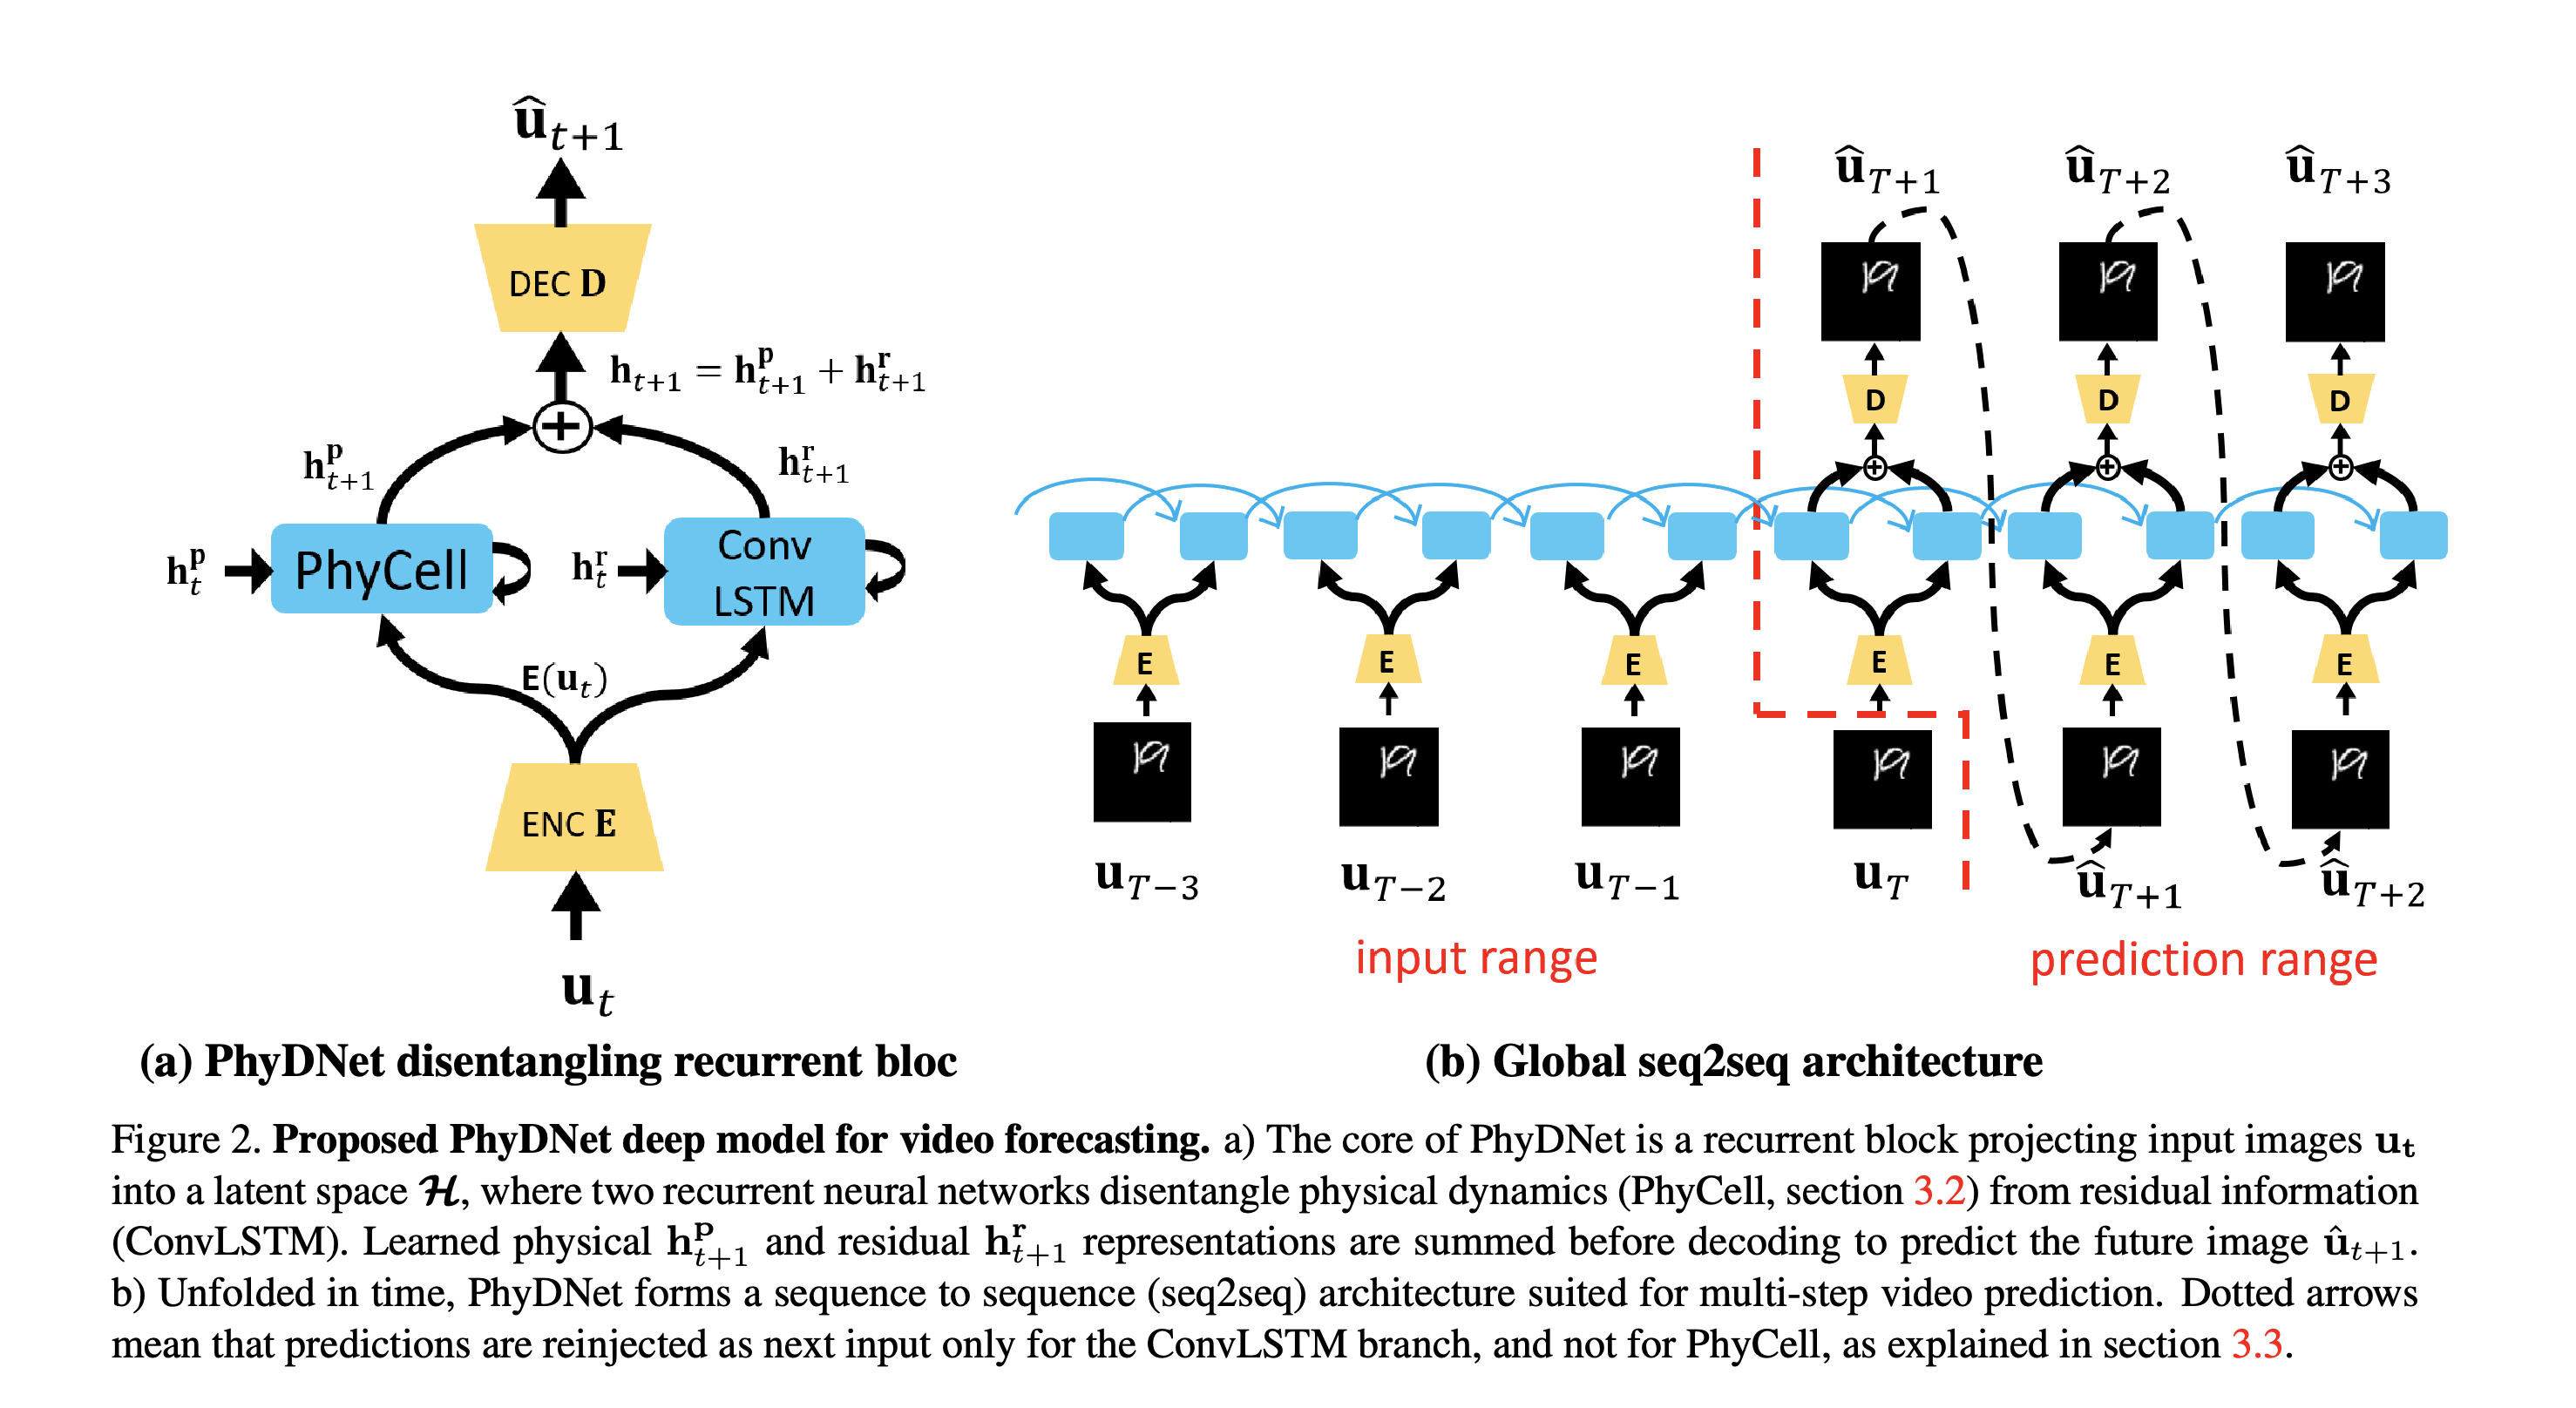
\includegraphics[width=0.8\textwidth]{images/phydnet.png}

\section{\citeall{Linial2020GenerativeUnknowns}}

Similar formulation like DSSM \cite{Miladinovic2019DisentangledRepresentations}. They use an ODE solver to propagate the state-space. Since this needs to be differentiable they use the RK4 from NeuralODE \cite{Chen2018NeuralEquations}. They also use "grounding" i.e. they use ground truth state-space to inform the latent space but only with low number of "labels" like 1 or 5 pc. Similar to what I want to do with length but they do it with the state space.

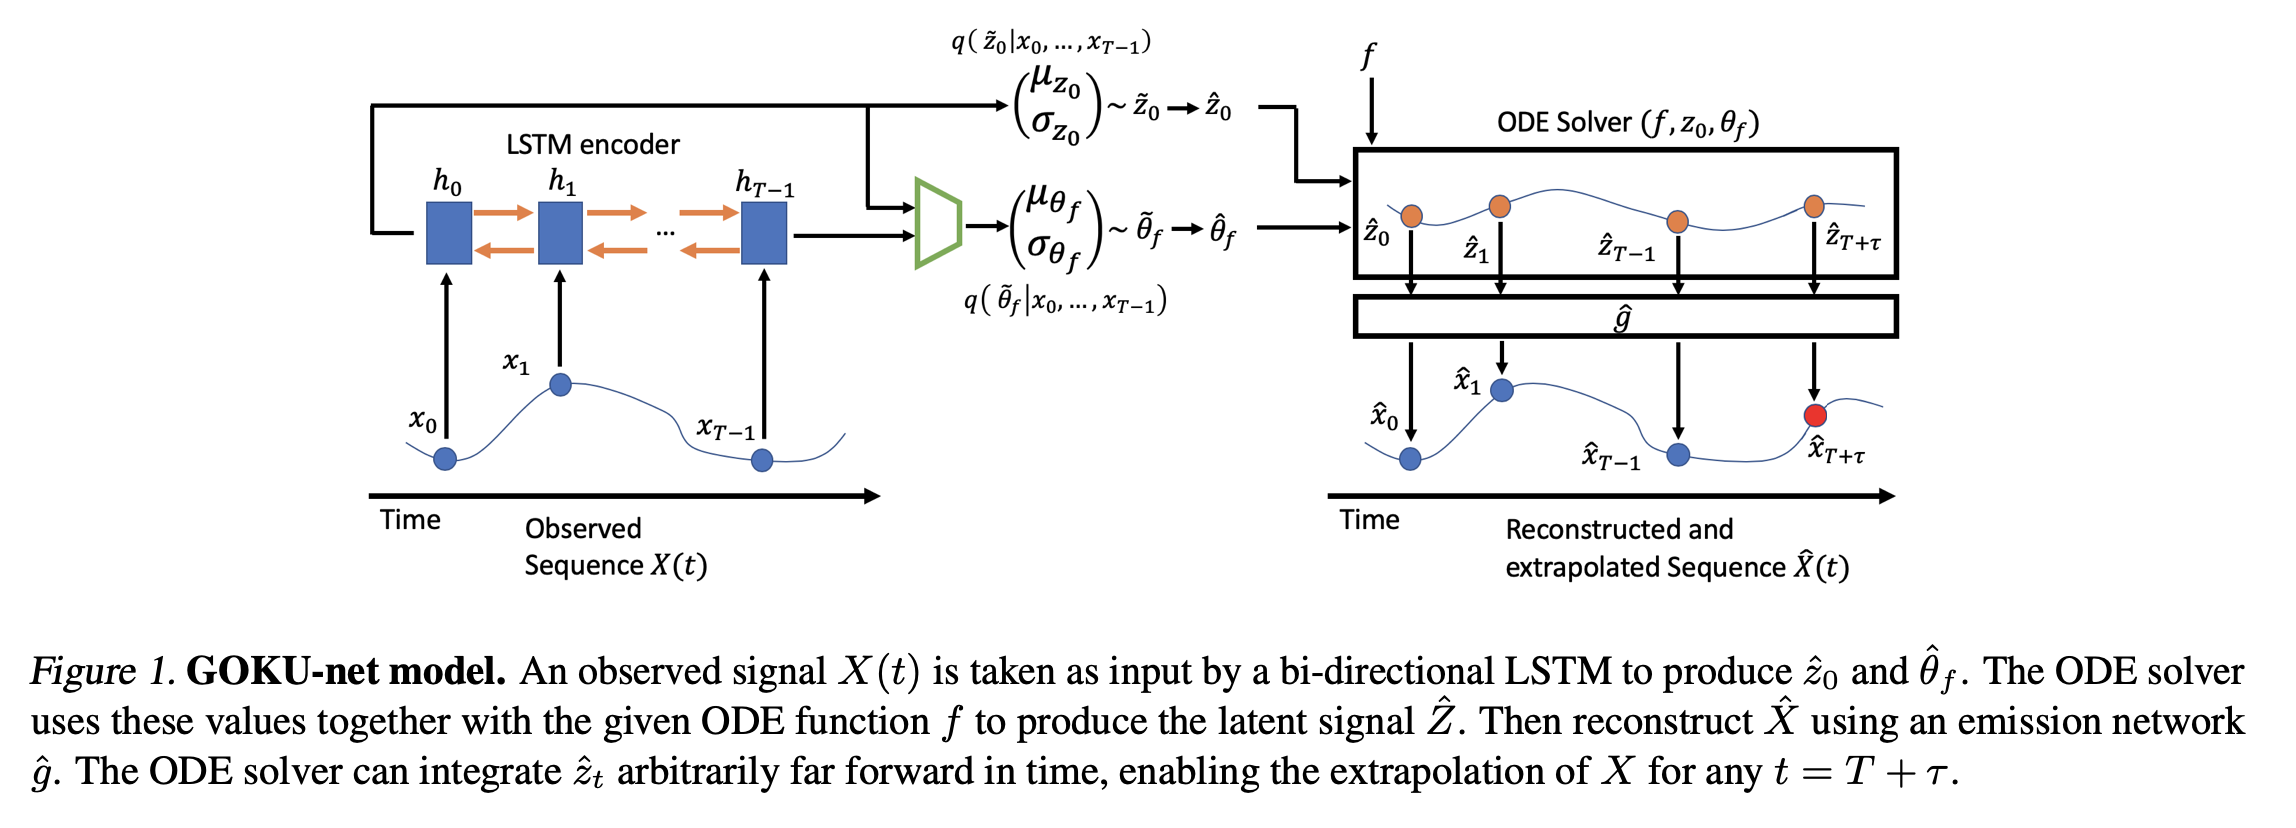
\includegraphics[width=0.8\textwidth]{images/goku.png}


\section{\citeall{Sun2019Test-TimeShifts}}

The idea is to use an auxiliary *unsupervised* loss to fine tune the model both during training and testing. For image classification such loss could be something as trivial as predicting rotation. The loss is not exactly *unsupervised* in the sense that we do have labels for it, but these are very cheap to generate. In physical systems that could be coming from domain knowledge e.g. energy conservation.

The network has two components. The first one is a shared component, we can think of it as a feature extrator. On top of this extractor there are two heads, one for the supervised and another for the unsupervised tasks. In previous work, the unsupervised loss was used in training only \cite{Hendrycks2019BenchmarkingPerturbations} and has showed that it increases the robustness in the main task, but this work also uses it to update the weights at training time before making a prediction. This work also makes another assumption that in test time the samples come from the same distribution. So in this case the keep the updates on the weights for each test sample (they call this online). 

This paper has a very good literature review for 
\uls
\li \textbf{Learning on test instances. }
``Shocher et al. (2018) pro- vide a key inspiration for our work by showing that image super-resolution could be learned at test time simply by trying to upsample a downsampled version of the input image. More recently Bau et al. (2019) improve photo manipula- tion by adapting a pre-trained GAN to the statistics of the input image.``
\li \textbf{Self-supervised learning} studies how to create labels from the data, by designing various pretext tasks that can learn semantic information without human annotations. E.g. predicting rotation, context, colorization etc.
\li \textbf{Non-adversarial robustness} studies the effect of corruptions, perturbations, out-of-distribution examples, and real- world distribution shifts \cite{Hendrycks2019BenchmarkingPerturbations}.

\li \textbf{Unsupervised domain adaptation (transfer learning)} studies the problem of distribution shifts, when an unlabeled dataset from the test distribution (target domain) is available at training time, in addition to a labeled dataset from the training distribution (source domain). The limitation of the problem setting, however, is that generalization might only be improved for this specific test distribution, which can be difficult to anticipate in advance.

\li\textbf{ Domain generalization} studies the setting where a meta distribution generates multiple environment distributions, some of which are available during training (source), while others are used for testing (target). With only a few environments, information on the meta distribution is often too scarce to be helpful, and with many environments, we are back to the i.i.d. setting where each environment can be seen as a sample, and a strong baseline is to simply train on all the environments.

\li \textbf{One (few)-shot learning} tudies how to learn a new task or a new classification category using only one (or a few) sample(s), on top of a general representation that has been learned on diverse samples.
\li \textbf{Continual learning} Continual learning (a.k.a. learning without forgetting) studies the setting where a model is made to learn a sequence of tasks, and not forget about the earlier ones while training for the later
\li \textbf{Online learning}. The basic setting repeats the following: receive xt, predict yˆt, receive yt from a worst-case oracle, and learn. Final performance is evaluated using the regret, which colloquially translates to how much worse the online learning algorithm performs in comparison to the best fixed model in hindsight.
\ule 

\section{\citeall{Alet2020Tailoring:Time}}

The extend the idea of test-time training from \cite{Sun2019Test-TimeShifts}, which they call tailoring. Furthermore they use meta-learning in the sense that during training they learn a model that will behave well on test-time with tailoring.


\printbibliography
\end{document}
